
\documentclass{article}
\usepackage{xcolor}
\usepackage{amsmath}
\usepackage{graphics}

\title{IT Internal }
\author{Rgukt Basar}
\date{\today}

\begin{document}
	\maketitle
	\center \textbf{Abstract}\\
	
	Answer any 2 of the following 3 questions. Time: 2 hours. Full marks 30.
	
	\flushleft{your abstract}
	\section{introduction}
	Reproduce the following sections in LaTeX:\\
	LaTeX is a high-quality typesetting system; it includes features designed for the production of technical
	and scientific documentation. LaTeX is widely used in academia for the communication and publication
	of scientific documents in many fields, including mathematics, computer science, engineering, physics,
	chemistry, economics, and political science.
	
	\subsection{Coloured Text}
	
	\large \textcolor{blue}{Introduction}\\
	
	\textcolor{blue}{This is the introduction section, highlighted in blue.}
	
	
	\large \textcolor{red}{Methodology}\\
	
	\textcolor{red}{This section discusses the methodology, highlighted in red.}
	
	
	\huge \textcolor{green}{Results}\\
	
	\small\textcolor{green}{This section presents the results, highlighted in green..}
	
	
	
	
	\subsection{Special Characters}
	LaTeX allows you to include special characters such as:\\
	Dollar sign: \$\\
	Ampersand: \& \\
	Percent: \% \\
	Hash: \#
	
	
	\subsection{Including Figures}
	To include figures, you first need to upload the image file named sample-image.jpg from your com-\\
	puter using the upload link in the file-tree menu. Then use the includegraphics command to include\\
	it in your document.\\
	\begin{figure}
		
		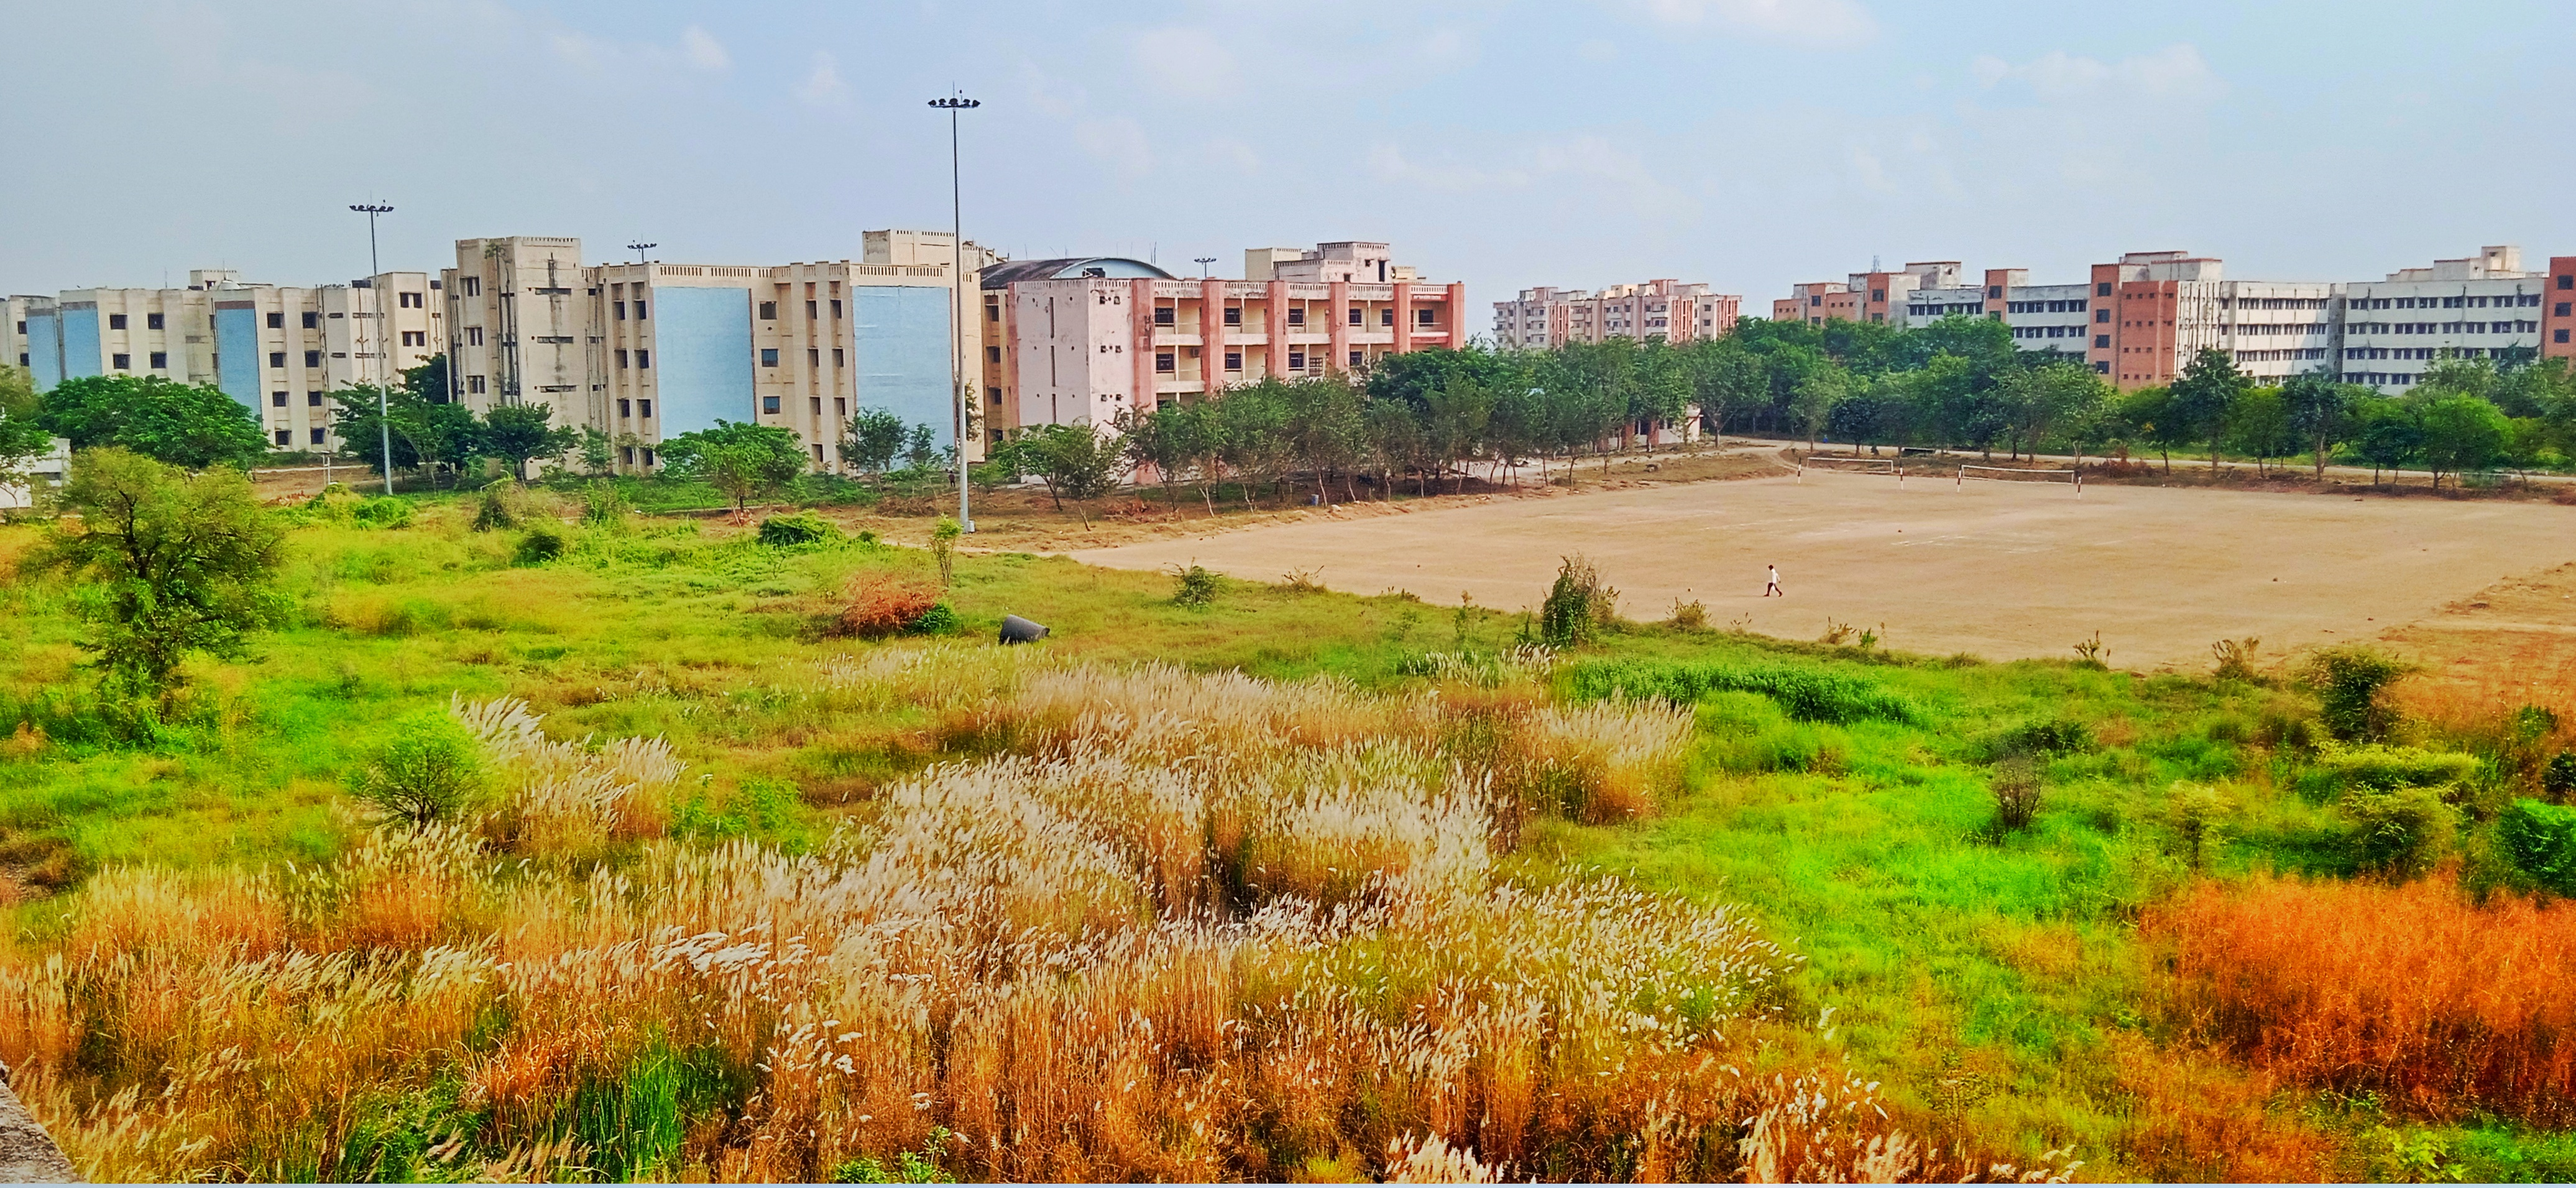
\includegraphics{rgukt.jpeg}
	\end{figure}
	
	\subsection{Creating Tables}
	Use the table and tabular environments for basic tables. Here’s an example:
	\begin{table}[h]
		\begin{tabular}{|c| c| c| }
			Item & Quantity & Price \\
			\hline
			Apples & 10 & \$1.50 \\
			
			Oranges & 5 & \$ 2.00
			
		\end{tabular}
	\end{table}
	
	
	\subsection{Mathematical Expressions}
	LaTeX excels at typesetting mathematics. Here is the quadratic formula inline: $ax^2 + bx + c = 0 $\\
	
	Displayed version:  $$ x = \frac{-b+\sqrt{b^2-4ac}}{2a} $$\\
	
	Sine and Cosine Addition Formulas:  $$ sin(a+b) = sinacosb+ cosasinb $$\\
	$$ cos(a+b) = cosasinb+ sinacosb $$\\
	Displayed version:    $$\int^a_b(fx)dx $$
	
	
	
	
	
	
	\subsection{Lists}
	You can make lists with automatic numbering . . .
	\begin{enumerate}
		\item First item,
		\item Second item,
		\item Third item
	\end{enumerate}
	You can also use bullet points with colored text:
	\begin{itemize}
		\item \textcolor{pink}{This text is magenta.}
		\item  \textcolor{yellow}{This text is magenta.}
		\item  This text is black.
		\item  \textcolor{gray}{This text is grey.}.
	\end{itemize}
	\subsection{HyperLinks}
	For more information, visit the \textcolor{blue}{LaTeX project website.}
	
	\subsection{Bibliography}
	To include references, you can use BibTeX. Here is an example citation \textcolor{blue}{[Doe24].}
	
	
	
	
	\vspace{3mm}
	
	\huge \textbf{References}
	\vspace{4mm}
	
	
	\small[Gre93] George D. Greenwade.
	14(3):342–351, 1993.
	The Comprehensive Tex Archive Network (CTAN).
	3
	TUGBoat,
	
	
\end{document}

\